\section{Social Networks Models}
\label{social_networks}

Field of social network analysis become one of the key field in  computer science's interdisciplinary research, so before introducing what kind of properties have been observed in real social network we have to briefly describe typical metrics and measurements used in social network analysis:
\begin{description}
\item [Grade] defined as the number of links (or relationships) to others that a network's node have\cite{newman:2010}. In networks represented as directed graph \emph{in-degree} and \emph{out-degree} are used to numerate incoming and outgoing links respectively. Grade one of the basic measure in social network analysis, but also keep a relevant role when the focus is on distribution of degree across nodes.
\item [Clustering] we can define clustering coefficient for a generic node $n_{i}$ as $\frac{number of pairs of neighbors of node_{i} that are connected}{number of pairs of neighbors of node_{i}}$. A whole network clustering coefficient could be calculated as $C=\frac{1}{n} \sum_{i=0}^{n} C_{i}$ \cite{citeulike:1580006}
\item [Average path length], measure the efficiency of the network in terms of how easy is transport an information from a node to another. It is defined as $\frac{\sum_{i,j}{d(i,j)}}{n\cdot (n-1)}$ where $i,j$ are network nodes, $n$ is the number of network nodes and $d(\cdot,\cdot)$ is the shortest path cost between two nodes ($0$ in case of not reachability or $i=j$). 
\item [Centrality] this kind of measures try to answer to the following question ``Which are the most important or central vertices in a network?''. Several kinds of centrality measures have been defined in order to characterize node's importance in the network, like:
\begin{itemize}
\item \emph{Degree Centrality}, which simply consider node's degree (as described previously)
\item \emph{Betweenness}, focus on how much a node is between other nodes, in particular can be defined as $ \frac{\sum_{j<k}{g_{jk}(i)}}{g_jk }$ where $g_{jk}$ is the number of shortest paths connecting $jk$ and
$g_{jk}(i)$ is the number that shortest path which includes node $i$.
\item \emph{Eigenvector centrality} it exploits different concept, this measure consider node centrality directly related to neighbours centralities\cite{newman:2010} (eg. if you have important neighbours you are much more important). It can be intuitively expressed as $C(i)=\sum_{k \in neighborhood}{\omega_{ki} \cdot C(k)}$ where $\omega_{ki}$ is the weight of the relationship (if present) and $C(\cdot)$ is the centrality.
\item \emph{Katz centrality} is a refinement of eigenvector centrality which enable to modulate the effect of neighbours centrality in node's centrality calculation. More formally we can express node-$i$ centrality as $C_{i}(\beta)= \sum_{j \in neighborhood}{(\alpha + \beta \cdot C_{j})\cdot \omega_{ij}}$ where $\beta$ is modulates the importance of neighbours centrality and $\alpha$ is a normalized constant.
\end{itemize}
\end{description}

\section{Small-World networks}
\label{sn_smallworld}
Real world network have been investigated deeply in past decades and similar characteristics have been observed in both biological, social, and computer networks (eg.web-pages or e-mails\cite{ebel02:_scale}). 
The common properties observed during investigations were fundamental for the development of networks models and consequential algorithm for realistic network generation - which are basic for setting up our experiment - so we need to introduce these properties:

\begin{description}

\item[Small-world property] real world networks are typically characterized  by the existence of shortcuts between different network areas, this contribute do maintain low average path length despite network size\cite{citeulike:481248}, speeding up the communication among otherwise distant nodes.

\item[Scale-free] degree distribution across network nodes follow a power-law such as $p(x) \sim x^{-\gamma}$ where $\gamma$ is a parameter typically between 2 and 3. An important property of this kind of distribution (which is an exponential distribution) is that it results to be scale invariant. Note that a distribution is scale invariant if $p(b \cdot x) = f(b) p(x)$, and if we consider a power-law distribution $p(c \cdot x) = (c \cdot x)^\gamma = c^\gamma f(x) \propto p(x)$.\\ 
Power-law distribution is also known as \emph{Pareto distribution} (80/20 principle) so roughly speaking we can observe that there are much more nodes with low-degree values rather than high-degree nodes.

\item[Community structures] real world networks are typically characterized by high\footnote{High clustering coefficient - and also low average path - are referred to the same measures taken from random graphs (eg. Erdos–Renyi model) } clustering coefficient's values, in fact fully connected sub-graphs (k-cliques) are a common motif in small-world networks\cite{citeulike:481248}. A recent analysis performed on data collected by an ad hoc massive multiplayer online game\cite{citeulike:6926207} have observed that high values of clustering are related to positive interactions, showing a correlation between communities and performance.

\end{description}

\subsection{Barabási-Albert model}
\label{sn_ba_model}
BA model\cite{citeulike:90557} is a network model based on two concept observable in real networks: growth, and preferential attachment. Older nodes become more popular during network growth and consequentially it's more probable that new nodes will be attach to them.\\
The algorithm consider degree as measure of popularity and use a probability of attachment calculated as follow: $p_{i} = \frac{k_{i}}{\sum_{j} k_{j}}$, where $p_i$ is the probability of creation of a connection (edge) between the new node and the node-$i$, $k_{i}$ is the node-$i$ degree, and $j \in 1 \cdots N$.\\
However BA-generated network does not provide a full small-word network. Despite the scale-free ($p(x)=x^{-3}$) degree distribution and the relatively low average short path ($\ell\sim\frac{\ln N}{\ln \ln N}. $), it doesn't capture typical motifs of real world networks: high clustering values and communities.\\
In fact in BA-model the clustering coefficient scales with network size in a power-law fashion, this behaviour is still different from small-world networks where clustering is independent from graph size.

\begin{algorithm}
\caption{BA network generation algorithm}
\label{sn_ba_alg}
\begin{algorithmic}
\FOR{$node_{i}$ such that $node_{i} \in graph$  } 
	\STATE $p_{i} = \frac{k_{i}}{\sum_{j \in 1\cdots N} k_{j}}$
	\IF{$random() \leq p_{i}$} 
	 	\STATE $connect(newnode,node_{i})$
 	\ENDIF
\ENDFOR
\end{algorithmic}
\end{algorithm}

\subsection{Watt-Strogatz model}
\label{sn_ws_model}
The WS-model\cite{citeulike:1580006} use a different approach for describing the small-world networks formation, it exploits a different concept related to observation of both random, regular, and small-world networks.\\
Considering the structure of small-word networks is possible to observe that they aren't neither regular nor random, so the main idea is to obtain a realistic network topology by moving from regular to random network by increasing randomness  in some way. The algorithm used for network generation\ref{sn_ws_alg} consists in two main steps: the creation of a regular lattice graph (with $K$ indicating the mean degree), and a successive random rewiring leaded by a probability of rewire $\beta$.

\begin{algorithm}
\caption{WS network generation algorithm}
\label{sn_ws_alg}
\begin{algorithmic}
\STATE
\COMMENT {Create a graph with N nodes each connected to K neighbours, K/2 on each side}\\
\STATE{$graph=createLatticeRing(nodes)$}\\
\COMMENT {Perform a random rewiring}
\FOR{$i$ from  $1$ to $N$ } 
	\FOR{$j$ from  $i+1$ to $N$ }
		\IF{$random()  \leq \beta$} 
	 		\STATE $connect(node_{i},node_{j})$
 		\ENDIF
 	\ENDFOR
\ENDFOR
\end{algorithmic}
\end{algorithm}

This model generates networks with logarithmic average path length, a clustering coefficient which depends on $K$ (not on size of graph), but does not generate a realistic - scale-free - degree distribution.

\subsection{Caveman model}
\label{sn_caveman_model}
Another interesting network model proposed in\cite{4149781} consists in a refinement of the classical caveman model, which is based on a set of connected sub-graphs wired each other in a regular lattice as shown in figure \ref{fig:caveman}.\\
 Once generated the base caveman graph, further random rewiring will be performed in a distinct way w.r.t. WS-model.\\
This model use the \emph{``s-metric''} as probability of rewiring: this metric aim to quantify the propensity of high-degree nodes to connect to other high-degree nodes, it is defined as $s(graph)=\sum_{i,j \in graph}{k_{i} \cdot k_{j}} $, where $k_{i}$ is the node-$i$ degree.\\
Whereas a probability is needed, this measure is used for normalizing single node's \emph{``s-value''}, so probability of rewiring results in $p(i,j) =\frac{k_{i} \cdot k_{j}}{\sum_{u,v \in graph, u \neq v}{k_{u} \cdot k_{v}}}$ with $i,j \in graph$, $i \neq j$.\\

\begin{figure}[h!]
	\begin{center}
    \label{fig:caveman}
    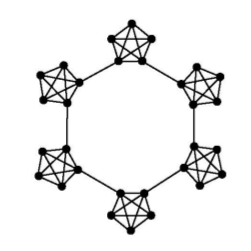
\includegraphics[scale=0.5]{img/caveman.png}
    \caption{Caveman network model (initial) with $m=5$ sub-groups}
  \end{center}
\end{figure}

\begin{algorithm}
\caption{Caveman enhanced generation algorithm}
\label{sn_ca_alg}
\begin{algorithmic}
\STATE
\COMMENT {Create a caveman graph with $m$ groups/communities}\\
\STATE{$graph=createInitialCavemanRing(nodes,m)$}\\
\COMMENT {Perform a random rewiring}
\FOR{$i$ from  $1$ to $N$ } 
	\FOR{$j$ from  $i+1$ to $N$ }
		\STATE $p_{i,j}=\frac{k_{i} \cdot k_{j}}{\sum_{u,v \in graph, u \neq v}{k_{u} \cdot k_{v}}}$
		\IF{$random()  \leq p_{i,j}$} 
	 		\STATE $connect(node_{i},node_{j})$
 		\ENDIF
 	\ENDFOR
\ENDFOR
\end{algorithmic}
\end{algorithm}

This model can generate networks with a high clustering coefficient, relatively low average shortest path, and - as reported in\cite{4149781} - with sufficient network size, a degree distribution very similar to power law distribution.
